\documentclass{article}
\usepackage{graphicx}
\usepackage{amssymb}
\usepackage{amsmath}
\usepackage{amsfonts}
\usepackage{latexsym}
\usepackage{hyperref}
\usepackage[all]{xy}
% \usepackage{feynmf}
\usepackage{slashed}
\usepackage{physics}
\usepackage{accents}
\usepackage{quoting}
\usepackage{afterpage}%for float placement
\usepackage{todonotes}%for notes-to-self, cuttext, etc.
\usepackage{adjustbox}
\usepackage{empheq}
\usepackage{verbatim}
% package used by \citep and \citet
\usepackage{natbib}

\usepackage{geometry}


 \geometry{
 a4paper,
 total={210mm,297mm},
 left=30mm,
 right=30mm,
 top=30mm,
 bottom=30mm,
 }

\begin{document}

\title{Predicting the Spread of Cointegrated Cryptocurrency Pairs with Long Short-Term Memory (LSTM) Neural Networks}
\author{Joshua Rosaler}
\date{}

\maketitle

\begin{abstract}
The application of Long Short-Term Memory (LSTM) neural networks to prediction of the spread of cointegrated cryptocurrency pairs is investigated. The Engle-Granger method is used to find cointegrated pairs among a set of seven major cryptocurrencies, and to calculate the stationary spread series for these pairs. The spread series is transformed for input into the LSTM network, and grid search with time series cross validation is used to select optimal hyperparameters, including batch size, number of neurons, and number of epochs of training. Performance on the test set is measured against a benchmark persistence forecast. Prior to cross validation, a preliminary grid search on the test set indicates that an ARMA(1,0,0) and a stacked LSTM marginally surpass performance of the benchmark forecast. However, for the range of hyperparameters explored, results of the cross validated LSTM model (from which the test set is withheld during hyperparameter selection) achieve results roughly equivalent to those of the benchmark performance on the test set. On the other hand, preliminary exploration of the spread series data indicate that cryptocurrencies are fertile ground for other cointegration strategies, such as non-parametric strategies that buy or sell the spread when it moves a certain number of standard deviations from the long-term average value. 
\end{abstract}

 

\section{Definition}

The main thread of implementation of this project is contained in the notebook Capstone\_Main.ipynb. The reader may wish to have this file open while reading this report. 


\subsection{Project Overview}
 
This project investigates the applicability of Long Short-Term Memory (LSTM) neural networks to the prediction of price spread movements of co-integrated cryptocurrency assets. In this introduction, I will provide background on LSTM networks, cointegration, and cryptocurrencies in order to contextualize the project's main aims. 

Long Short-Term Memory (LSTM) neural networks are a type of Recurrent Neural Network (RNN) that has recently had a lot of success in modeling sequence data, including in character-level language modeling, time series prediction, and speech recognition. RNNs differ from ordinary feedforward neural networks in several important ways: first, the data that they take as input is time-ordered, so that samples cannot be randomly shuffled during training as they can in other machine learning models, including feedforward networks; second, they have an internal state that can be used to ``remember" patterns occurring earlier in the sequence, which can be used in the prediction of future elements of the sequence. However, ordinary or ``vanilla" RNNs suffer from the so-called vanishing gradient problem, which limits how far back into the past they can remember. LSTM networks correct this problem through the use of an internal cell state which is updated by new data via certain gates. Given their ability to remember patterns in sequence data over long periods of time, it is natural to consider their application to the prediction of price movements in financial markets. 

Pairs trading is a class of market-neutral trading strategy - i.e., a strategy whose profitability does not depend on the rise or fall in price of assets being traded, but rather on the relative price between different assets. Thus, the idea is in a certain sense to trade on the relationship or spread between different assets rather than directly on the prices of the assets themselves. Cointegration is a statistical technique that lies at the foundation of a particular type of pairs trading known as statistical arbitrage. A set of price series for different assets are said to be cointegrated if a linear combination of these assets, known as the spread, is stationary. The spread itself can be bought and sold as though it were an asset. Informally, stationarity of the spread series requires that the statistical properties of the series, such as mean, variance, and autocorrelation, do not change over time as one moves forward or backward in the sequence. Stationarity is a useful property for trading because it implies mean reversion: if the value of the series lies well above (e.g. a standard deviation) the mean, this enables us to predict that the price will very likely decrease in the future and suggests that we should sell or short the spread; likewise, if the value of the series lies well below the mean, this enables us to predict that the price will very likely rise in the future and suggests that we should buy the spread. 

Cryptocurrencies are a particular type of asset to which one can apply the techniques of pairs trading. They are a new form of digital currency that has been available for public trading for less than a decade, since Bitcoin, the most widely known cryptocurrency, began trading in 2009.  Since then, other cryptocurrencies known as altcoins, such as Ethereum, Litecoin, Monero, Dash, Ripple, and Bitcoin Cash, have come about. Currently, there exist more than a thousand different types of cryptocurrency. Different cryptocurrencies may differ in the details of the contracts that they allow and the manner in which they are exchanged. For example, Ethereum was invented to allow for the possibility of ``smart contracts," which allow for exchanges of money, property, and other valuable assets without requiring both parties to put their trust in a middle man. Cryptocurrencies are traded on special cryptocurrency exchanges, such as Coinbase. Cryptocurrencies are based on blockchain technology, which allows for a decentralized, anonymous ledger of transactions and, unlike ordinary currency, does not require a government, bank, or other institution with access to a record of your purchases. 

The application of pairs trading strategies in cryptocurrency markets remains a relatively under-explored subject. The question of whether cointegration techniques can be usefully applied in this realm therefore has the potential to reveal a new source of profitable trades. Likewise, the question of whether machine learning techniques, and LSTM networks in particular, can be employed to facilitate pairs trading in cryptocurrency markets also seems worthy of investigation. 

\subsection{Problem Statement}

This project seeks to answer the question:

Can LSTM neural networks be used to enhance cointegration-based pairs trading strategies?

Specifically, the project investigates the possibility that LSTM networks can be used to predict the movement of the spread of a pair of cointegrated cryptocurrency price series on the basis of historical price data alone, in order to improve the strategy for buying and selling the spread. An important  initial step is to find cointegrated pairs of cryptocurrency assets based on daily closing price history, and to compute the spread for these pairs. Focusing on the spread for a specific pair, I examine whether the LSTM network provides a reliable 1-day forecast of the spread. 

The use of LSTMs in forecasting cryptocurrency spread series will be treated here as a regression problem, in which the LSTM network takes some number $p$ of lags (previous values) of the spread series, and outputs the value of the series one step into the future. The network weights will be trained using a variant of gradient descent; in the context of recurrent neural networks, these gradients are computed through the variant of the back propagation procedure known as back propagation through time. The training and validation procedure will make use of time series cross validation, a variation of K-fold cross validation that accommodates the ordered nature of samples in a time series dataset.  

The application of LSTMs to forecasting of stock prices has had moderate success in some cases, and this project seeks to determine how they fare in predicting price spreads of cointegrated assets. My expectation prior to performing the analysis was that they should provide some improvement over the benchmark persistence forecast described below. 



\subsection{Metrics}

Forecasting of spreads series $s_{1}, s_{2}, ..., s_{N}$ is treated here as a regression problem. The effectiveness of the forecasting models will be measured in terms of root mean squared error (RMSE), a standard measure of performance of regression models. Given test observations, 
$\{(X_{1}, y_{1}), (X_{2}, y_{2}), ...,  (X_{N}, y_{N}) \}$ where $X_{i} = [s_{i}, s_{i-1}, ..., s_{i-p}]$ and $y_{i} = s_{i+1}$,
the RMSE is computed as the square root of the average of squared deviations between the forecasted value $\hat{y}_{i}(X_{i})$ and the true value $y_{i}$:

\begin{align}
RMSE(\boldsymbol{\hat{y}}, \boldsymbol{y}) = \sqrt{\sum_{i=1}^{N} \left(\hat{y}_{i}(X_{i}) - y_{i}\right)^{2} },
\end{align}

\noindent where $\boldsymbol{\hat{y}} \equiv (\hat{y}_{1}, ... , \hat{y}_{N})$, $\boldsymbol{y} \equiv (y_{1}, ... , y_{N})$. This metric provides a useful measure of deviation between predicted and actual values of the series. Other metrics such as the mean absolute error can also be used, but do not possess the nice differentiability properties of the RMSE (which become important when computing gradients during training). For this reason, it is usually the RMSE (or simply the MSE) that is used as a measure of regression model's performance. 


 The base model against which the test set RMSE of the LSTM model will be compared is a basic persistence forecast model, which predicts that the next day's price of the spread will be equal to the current day's spread price. At a bare minimum, the test RMSE of the LSTM should lie below the test RMSE of the persistence model in order to be useful in pairs trading strategies. 








\section{Analysis}

\subsection{Data Exploration}

The cryptocurrency price data was drawn from Kaggle: \url{https://www.kaggle.com/sudalairajkumar/cryptocurrencypricehistory/version/13}. The dataset consists of open, high, low, close, volume, and market cap data for eighteen different cryptocurrencies. 
To keep the analysis manageable, and to ensure sufficient training data, I focused on a subset of the available cryptocurrencies: Bitcoin, Ethereum, Litecoin, Dash, Monero, Nem, and Ripple. They were chosen in large part because they have existed for a sufficiently long time that a substantial amount of training data exists for all of them. The earliest date for which price histories exist for all of these currencies is August 7, 2015. The last date for which price data exists for all currencies is Feb. 20, 2018. I also chose to focus specifically on closing price data because this provides a regular daily sampling of the price data, and to focus the analysis on whether LSTM networks are capable of predicting future prices on the basis of past price data alone (see Fig. \ref{FigSample}). Basic descriptive statistics of the price data are plotted in Fig. \ref{FigStats}.






\begin{figure}[]
\includegraphics[scale=0.50]{/Users/jrosaler/Dropbox/Extra/"Udacity Capstone"/"Capstone Submission 3"/Cryptos_head.pdf}
\caption{A sample of the dataframe of cryptocurrency prices considered for cointegration. }
\label{FigSample}
\end{figure}

\begin{figure}[]
\includegraphics[scale=0.50]{/Users/jrosaler/Dropbox/Extra/"Udacity Capstone"/"Capstone Submission 3"/Cryptos_describe.pdf}
\caption{Summary of dataframe statistics. }
\label{FigStats}
\end{figure}



\subsection{Exploratory Visualization}

Plotting the data for the seven listed currencies shows a dramatic rise in price of all cryptocurrencies starting around Apr. 2017 (see Fig. \ref{FigPrices}). Since the price levels of the different currencies differed dramatically, with Bitcoin much higher than the rest, the price series were normalized through division by their initial values. Zooming in on the period between July 2017 and Feb. 2018, one sees that the different cryptocurrencies exhibit a strong tendency to move together, suggesting that they may be fertile ground for cointegration strategies (see Fig. \ref{FigCumRet}). Returns were also plotted, and exhibit fluctuating volatility for most of the currencies.  


\begin{figure}[]
\includegraphics[scale=0.70]{/Users/jrosaler/Dropbox/Extra/"Udacity Capstone"/"Capstone Submission 3"/Prices.png}
\caption{Price history shows a dramatic rise in price across different cryptocurrencies in the second half of 2017. }
\label{FigPrices}
\end{figure}

\begin{figure}[]
\includegraphics[scale=0.70]{/Users/jrosaler/Dropbox/Extra/"Udacity Capstone"/"Capstone Submission 3"/CumReturns.png}
\caption{Strong co-movement of cumulative returns suggests that cryptocurrencies may be fertile ground for cointegration strategies. }
\label{FigCumRet}
\end{figure}

%Plotting the data for the seven listed currencies shows a dramatic rise in price of all cryptocurrencies starting around Apr. 2017 (see Fig. \ref{FigPrices}) . Since the price levels of the different currencies differed dramatically, with Bitcoin much higher than the rest, the price series were normalized through division by their initial values. Zooming in on the period between July 2017 and Feb. 2018, one sees that the different cryptocurrencies exhibit a strong tendency to move together, suggesting that they may be fertile ground for cointegration strategies. 
%Returns were also plotted, and exhibit fluctuating volatility for most of the currencies. A pair plot of the returns confirms a strong correlation between many pairs of cryptocurrencies, an indicator of potentially fertile territory for cointegration.

\subsection{Algorithms and Techniques}

\subsubsection{Cointegration Techniques}

A set of assets $X_{1}, ... , X_{N}$ is set to be cointegrated if there exists a linear combination 

\begin{align}
S = b_{1} X_{1} + ... + b_{N} X_{N}
\end{align}

\noindent of these assets that is stationary. The vector $(b_{1}, ..., b_{N})$ of coefficients is known as the cointegration vector. A stochastic process generating a time series is stationary if its unconditional joint probability distribution is unchanged when shifted in time. As a consequence, quantities such as the mean and autocovariance (covariance between values of the series separated by some number of time steps) of the process are left unchanged when the series is shifted in time. A stochastic process is said to be weakly stationary if its mean and autocovariance are left unchanged by such shifts. The series $S(t)$ is sometimes known as the spread of the assets, and assuming that all assets $X_{1}, ... , X_{N}$ can be bought, sold, and shorted, can be traded as an asset itself. Stationary series have the useful property that they are mean reverting and so predictable: if they deviate below the mean, one can reliably predict that they will rise toward the mean, and if they deviate above the mean, one can reliably predict that they will drop back toward the mean. 

There are several different methods for finding cointegrated combinations of assets, including the Engle-Granger two-step method, the Johansen test, and the Philips-Ouliaris cointegration test. We focus here on applying the Engle-Granger method to cointegration of two assets. The two steps of the Engle-Granger method are as follows:

\begin{itemize}
\item Perform a linear regression of one asset against the others. 
\item Test the residuals for stationarity, for example using the augmented Dickey-Fuller test.
\footnote{The augmented Dickey-Fuller test tests the null hypothesis that a unit root is present in a given time series sample. The alternative hypothesis is that the series is stationary.
} 
\end{itemize}

\noindent For the case of two assets $X_{1}$ and $X_{2}$, the linear regression step yields 

\begin{align}
S(t_{i}) = X_{1}(t_{i}) - b X_{2}(t_{i}) = \mu + \epsilon(t_{i})
\end{align}

\noindent where $i = 1, ..., N$ (indicating $N$ observations for each component series), $b$ is the slope parameter, which also determines the relative weighting of the assets in the appropriate linear combination, and $\mu$, the y-intercept, is the mean value of the spread series. If the residuals $\epsilon(t_{i})$ are stationary, then $X_{1}$ and $X_{2}$ are cointegrated. For further discussion of cointegration, see \cite{vidyamurthy2004pairs}. 

Financial assets that are cointegrated often lie in the same industry and their prices are subject to the same underlying factors. On the whole, they tend to move together, and their difference - or other suitable linear combination - can be treated as stationary. 



\subsubsection{Non-Parametric vs. Parametric Methods in Pairs Trading}

In \cite{vidyamurthy2004pairs}, Vidyamurthy draws a fundamental distinction between ``parametric" and ``non-parametric" approaches to pairs trading. Parametric approaches use an explicit model, such as a classical linear ARIMA model or in our case a non-linear LSTM model, to predict the movement of the spread series. Non-parametric approaches do not use any model. An example of a non-parametric approach would be to predict that the price of the spread will fall when it is one standard deviation above its mean, and that it will rise when it is one standard deviation below; no model is involved here. 

\subsubsection{Cointegration of Cryptocurrencies}

The main source on cointegration of cryptocurrencies used in this project is a paper titled ``Constructing Cointegrated Cryptocurrency Portfolios for Statistical Arbitrage" by Leung and Nguyen's 2018 article, \cite{leung2018constructing}. They investigate four cryptocurrencies - Bitcoin, Ethereum, Litecoin, and Bitcoin Cash - measuring the performance of spread portfolios constructed using the Engle-Granger and Johansen cointegration methods. They find the Engle-Granger approach to be more profitable as it results in a spread series that is more rapidly mean reverting. They form the spread portfolio by performing ordinary least squares multiple linear regression of the Bitcoin price series against the other three. Calculating the autocorrelation function (ACF) and partial autocorrelation function (PACF), they determine that an ARMA(1, 0, 0) = AR(1) model best fits the spread when compared to different orders of ARIMA(p,d,q) model. They adopt a trading strategy in which they go long the spread or exit a short position when the spread $S < \mu -  c * \sigma$ and short the spread or exit a long position when $S > \mu +  c * \sigma$, where $\mu$ is long-run mean $\sigma$ the standard deviation of the series, and $c$ is a constant of order one. From backtesting they determine that $c = 1.5$ is the optimal value for maximizing profit, after testing multiple thresholds associated with different values of $c$. 


\subsubsection{Recurrent Neural Networks}

Recurrent neural networks (RNNs) take as input the network's hidden state $h_{t-1}$ at the previous timestep and the external input $x_{t}$ at the current timestep. The network first multiplies the external input  $x_{t}$ by a $n \times m$ matrix $W_{hx}$, where $m$ is the number of external inputs (e.g. number of lags), and $n$ is the number of neurons in the hidden state. To this it adds the product of the $n \times n$ matrix $W_{hh}$ with the previous hidden state $h_{t-1}$, as well as an $n \times 1$ bias term $b$. A $\tanh$ activation function is then applied element-wise to this sum: 

\begin{align}
h_{t} = \tanh(W [h_{t-1}, x_{t}] + b),
\end{align} 

\noindent where $W [h_{t-1}, x_{t}] \equiv W_{hh} h_{t-1} + W_{hx} x_{t}$ . $h_{t-1}$ is thus both the output of the network at time $t-1$ and input to the network at time $t$.  The same weight matrices $W_{hh}$ and  $W_{hx}$ are used across different time steps. 

\begin{figure}[]
\includegraphics[scale=0.40]{/Users/jrosaler/Dropbox/Extra/"Udacity Capstone"/"Capstone Submission 3"/LSTM3-SimpleRNN.png}
\caption{A vanilla recurrent neural network (RNN). The network uses the same weights across different time steps, and takes as input both the hidden state from the previous time step $h_{t-1}$ and the external input $x_{t}$ at the current time step. Image credit: Christopher Olah, \url{http://colah.github.io/posts/2015-08-Understanding-LSTMs/}. }
\label{LSTMChain}
\end{figure}

The hidden state $h_{t}$ of the RNN enables the network to ``remember" patterns earlier in the sequence. However, their capacity to do so is limited by the so-called vanishing gradient problem, which arises during training of the network, which is performed through a variation of back propagation known as backpropagation through time. For further detail, see for example, \cite{olah2015understanding}, \cite{goodfellow2016deep}.





\subsubsection{LSTM Neural Networks}

The following explanation of LSTM neural networks draws primarily on \cite{olah2015understanding}. An LSTM neural network is an elaborate type of recurrent neural network (RNN) that addresses the vanishing gradient problem through the use of a second hidden state known as the cell state $C_{t}$, in addition to the hidden state $h_{t}$ that occurs in ordinary RNN's. This cell state enables the network to remember sequence patterns over many time steps, and is updated through the use of various gates. In this subsection, we will focus on the mathematical relationships that relate the input and output of the LSTM. Detailed explanation of how these relationships serve to address the vanishing gradient problem can be found for example in  \cite{goodfellow2016deep}. Roughly speaking, though, the additional cell state permits gradient to flow relatively unchanged during backpropagation from later to earlier time steps without being diminished by many factors of the weight matrix $W$ (as occurs in the case of ordinary RNN's). The cell state update process, denoted by the upper horizontal flow line in Fig. \ref{LSTMChain}, has been likened to a ``superhighway" across gradients can flow undiminished during back propagation.  



\begin{figure}[]
\includegraphics[scale=0.40]{/Users/jrosaler/Dropbox/Extra/"Udacity Capstone"/"Capstone Submission 3"/LSTM3-chain.png}
\caption{An LSTM Neural Network solves the problem of vanishing gradients that arises in ``Vanilla" recurrent neural networks through the use of a cell state and gates that determine how the cell state is updated at each time step. Image credit: Christopher Olah, \url{http://colah.github.io/posts/2015-08-Understanding-LSTMs/}. }
\label{LSTMChain}
\end{figure}


The cell state $C_{t}$ at time $t$ is computed as the sum of the element-wise product $*$ of a ``forget gate" $f_{t}$ with the previous cell state $ C_{t-1}$ and the element-wise product of an ``input gate"  $i_{t}$ with a candidate adjustment $ \tilde{C}_{t}$ to the cell state: 

\begin{align} \label{CellUpdate}
C_{t} &= f_{t} * C_{t-1} + i_{t} * \tilde{C}_{t}, \\
\end{align}

\noindent where,


\begin{align}
f_{t} &= \sigma(W_{f} [h_{t-1}, x_{t} ] + b_{f}) \\
i_{t} &= \sigma(W_{i} [h_{t-1}, x_{t}] + b_{i} ), \\
\end{align}

\noindent $\sigma(x) = \frac{1}{1 + e^{-x}}$, and 

\begin{align}
\tilde{C}_{t} &= \tanh(W_{C} [h_{t-1}, x_{t}] + b_{C}). \\
\end{align}

\noindent The update to the hidden state $h_{t}$ is performed according to 

\begin{align}
o_{t} &= \sigma(W_{o}  [h_{t-1}, x_{t}] + b_{o}) \\
h_{t} &= o_{t} * \tanh{C_{t}}. 
\end{align}

\noindent The various weights $W$ and biases $b$ appearing in these relations serve to parametrize the various sub-networks in the LSTM layer, and are learned during training through back propagation and a variation of gradient descent. The sigmoid functions $\sigma$ ensure an output between $0$ and $1$; in relation (\ref{CellUpdate}), they determine which components of the previous cell state $C_{t-1}$ are maintained and which components of the candidate update $\tilde{C}_{t}$ are incorporated into the new cell state. 

Like layers in an ordinary feed forward neural network, LSTM layers can also be stacked, so that the output $h_{t}$ of the first LSTM layer is fed in as input into a second LSTM layer at the same time. 






%\begin{align}
%f_{t} &= \sigma(W_{f} [h_{t-1}, x_{t} ] + b_{f}) \\
%i_{t} &= \sigma(W_{i} [h_{t-1}, x_{t}] + b_{i} ) \\
%\tilde{C}_{t} &= \tanh(W_{C} [h_{t-1}, x_{t}] + b_{C}) \\
%C_{t} &= f_{t} * C_{t-1} + i_{t} * \tilde{C}_{t} \\
%o_{t} &= \sigma(W_{o}  [h_{t-1}, x_{t}] + b_{o}) \\
%h_{t} &= o_{t} * \tanh{C_{t}}
%\end{align}








\subsubsection{Recurrent Neural Networks in Pairs Trading}

Given the past success of LSTM neural networks at identifying patterns in sequential data such as speech and text data, it is reasonable to imagine that they might also be of use in the prediction of financial price series data. 
%However, after finding a few cases where people had tried this, and after trying it myself, it appears that LSTM networks provide only marginal, if any, benefit when applied directly to the prediction of stock or spread series prices based only on previous prices as input. More information than past values of the spread series may be needed to improve the effectiveness of the LSTM. 
The notion of applying RNNs to predicting the spread of a co-integrated pair of assets is explored in \cite{dunis2006modelling} and \cite{van2017pairs}. In \cite{dunis2006modelling}, Dunis \textit{et al} apply various types of neural network, including multi-layer perceptron (MLP) and ordinary vanilla RNNs, to forecasting the change in the gasoline-crack spread. In each case, the network takes as input some positive integer number $p$ of lags of the differenced spread series. As output it produces the value of the change in spread at the next time. The network is trained so as to minimize mean squared error between predicted and actual changes in spread. The authors experiment with various models and trading filters, which dictate when to buy and sell the spread. Measured in terms of out-of-sample returns, the RNN with threshold filer was shown to have roughly 16 \% annual returns out-of-sample after transaction costs have been taken into account. 
 
Drawing on this analysis, \cite{van2017pairs} applies LSTMs to forecasting the change in the spread between pairs of exchange traded funds (ETFs) in various sectors. Like \cite{dunis2006modelling}, he takes a positive integer number p lags of the spread series for a pair and as output the value of the spread at the next time. He finds that the best performance, as measured in terms of mean squared error on the test set, is given for both the LSTM and FNN by a network with 5 lags, 2 hidden layers, and 3 hidden units per layer. He finds that the LSTM applied with Dunis et al?s threshold filter outperforms other models using the same filer, including a feedforward neural network (FNN), yielding an excess return of about 11 \% over a two-year trading period on a portfolio of the top 5 cointegrated ETF pairs. 

\subsection{Benchmark Model}

The benchmark model for 1-day forecast of the Ethereum/Litecoin spread was taken to be a persistence model, which predicts that the next day's spread will be equal to the previous day's. 
On the test set, this model achieved an RMSE of 14.353. This value sets the benchmark for performance of the LSTM and any other forecasting models on the test set. 


\section{Methodology}

\subsection{Data Preprocessing}

The data consists of 929 days of closing price data for the seven cryptocurrencies. To ensure a large amount of training data, and also that the training set was an evenly divisible number to allow for stateful LSTM networks (where the batch size must divide evenly into the size of the training set), the first 800 days of data were taken as the training set and the last 129 as the test set. From this stage of the analysis onward, the test set is removed from consideration until the final validated LSTM model and benchmark model are tested. 

The spread series data to which the LSTM is applied comes initially as a univariate time series, which is obtained as a linear combination of the price series data for two distinct cryptocurrencies via the cointegration procedure described below. Since time series prediction is a supervised learning problem, taking some number of lags of the series as input and the next value of the series as output, the data must be transformed to reflect this. This is accomplished by the function $timeseries\_to\_supervised$ (see the notebook Capstone\_Main.ipynb), which associates to each time step a single feature for each of the $p$ lags of the time series, and a label given by the value of the time series at the next step. In preparing data for use in an LSTM, it is also prudent to ensure that the data are standardized to particular scale, such as the interval [-1, 1], and that they are stationary. The scale transformation is performed by the function scale, and can be inverted by the function $invert\_scale$, which is used during forecasting. The spread series is already stationary by virtue of the nature of the cointegration procedure. However, ( \cite{dunis2006modelling} nevertheless recommended to difference the spread series prior to inputting it into the LSTM network. The differencing is performed by the function $difference$, and is inverted by the function $inverse\_difference$. The code for these transformations has been adapted from Brownlee's blog posts on time series forecasting with machine learning - in particular, \cite{brownlee2016time}. 

As an additional piece of data preparation, the training set is smoothed using a rolling average mean over a 5-day window, in order to remove some of the noise that may disrupt the training of the LSTM. However, it was not found that this resulted in significant improvement of network performance on the test set. 

\subsection{Implementation}

\subsubsection{Cointegration}

Cointegrated pairs are identified solely on the basis of the training data, in order to avoid look-ahead bias. The code for finding co-integrated pairs and checking them for stationarity was adapted from the Quantopian Jupyter notebook lectures on pairs trading and cointegration: \url{https://www.quantopian.com/lectures/integration-cointegration-and-stationarity} \cite{quantopian_cointegration}.

Here, the Engle-Granger two-step method of cointegration was used. In the Jupyter notebook for this project, the method is implemented via the functions $find\_cointegrated\_pairs$, and $check\_for\_stationarity$, which were adapted from the Quantopian notebooks. The function $find\_cointegrated\_pairs$ accepts a data frame of price histories and checks each pair of assets for cointegration using the statsmodels $coint$ function. It returns two matrices, one of p-values associated with each pair, and the other of t-statistic scores indicating the strength of the cointegration relationship. In addition, it returns a list of pairs for which the p-value falls below the specified threshold of $.001$.  

The function  $check\_for\_stationarity$ accepts a single price series, corresponding to the residuals obtained through ordinary least squares regression of one member of a pair against the other member of the same pair, as well as a cutoff for the p-value that results from the stationarity test. It returns True if the p-value resulting from an Augmented Dickey-Fuller test of the series is lower than the cutoff and False otherwise. This function uses the statsmodels adfuller function to check whether the input series is stationary. 

Four co-integrated pairs were identified by these functions with a p-value threshold of .001: Bitcoin/Monero, Ethereum/Litecoin, Ethereum/Nem, Litecoin/Nem. The p-value was chosen to be small - it is often chosen at the significantly larger value of .05 - to select for pairs with a strong cointegration relationship. I also attempted to look for pairs based on the log price histories rather than the price histories themselves, but found that this yielded no candidate pairs. 

The spread series for the four cointegrated pairs were plotted, and all showed a simultaneous and dramatic increase in volatility around April 2017, which coincides with start of the dramatic price increase across different cryptocurrencies. From this date until the end of the training set in October 2017, all four spread series show strong oscillations around the mean spread, indicating viability for pairs trading. The large oscillations suggest that all four spreads are good candidates for a simple non-parametric strategy in which one goes or stays short the spread when it deviates by, say, a standard deviation above the mean, and goes or stays long the spread when it deviates by a standard deviation below the mean (the optimal threshold should be determined by backtesting). However, we focus here on the parametric strategy that seeks to explicitly model the movement of the spread series using models such as LSTM and ARIMA. 

To analyze the applicability of LSTM models for spread series prediction, I chose to focus specifically on the spread series of the co-integrated pair with the smallest p-value, which turned out to be the Ethereum/Litecoin spread (see the associated Jupyter notebook for plots of the four spread series).

\subsubsection{Preliminary Fits and Tests of LSTM and ARIMA forecast models}

The code for training and forecasting the spread using the LSTM and ARIMA models, and for evaluating these models on the test set, is adapted from Jason Brownlee's blog posts. The following posts were particularly useful:

\

\noindent \url{https://machinelearningmastery.com/time-series-forecasting-long-short-term-memory-network-python/}

\noindent \url{https://machinelearningmastery.com/arima-for-time-series-forecasting-with-python/}.

\

\noindent The stacked LSTM architecture is adapted from Siraj Raval's Github page,

\

\noindent \url{https://github.com/llSourcell/How-to-Predict-Stock-Prices-Easily-Demo}.

\

\noindent Jakob Aungier's blog post on using LSTMs to predict sine waves and stock prices was another useful reference on this subject:  

\

\noindent \url{https://github.com/jaungiers/LSTM-Neural-Network-for-Time-Series-Prediction}.

\

When initially getting my code to work, I worked with only a train and test set, but no validation set. In this context, I considered three models: Vanilla (single hidden layer) LSTM, stacked LSTM, and ARIMA. For the single-layer and stacked LSTMs, I experimented with several batch sizes, epoch numbers, and numbers of neurons in the hidden layers. The number of epochs was originally in the range $50 - 3000$ (where the upper limit was drawn from Brownlee's LSTM post above), while the batch size was in the range $100 - 200$, and the number of neurons in each layer was varied between $10$ and $64$. The window size used, corresponding to the number of lags input into the models at each time step was kept fixed at $100$. Initially the batch sizes were kept to factors of $800$, the size of the training set, to ensure compatibility with a stateful LSTM. However, I subsequently found that making the LSTM stateless did not yield a substantial change in the quality of the model's predictions and allowed for more flexibility in choosing the batch size.  

In testing the LSTMs performance on the test set, a walk-forward validation procedure was used in which the prediction for the next time step in the test set was forecast on the basis of 100 lags. Model parameters were kept to values fixed by fitting to the training set. In principle, one could update the model parameters at with each new observation in the test; however, in the case of the LSTM this would be cumbersome and computationally expensive, without any likelihood of a dramatic increase in performance. The function $fit\_lstm$ was used to fit the LSTM model, while $forecast\_lstm$ was used to make the forecasts on the basis of the trained model. 

The preliminary testing also investigated the performance of ARIMA models in forecasting the Ethereum/Litecoin spread. The appropriate order of the ARIMA model was determined by a grid search on the test set using the functions $evaluate\_arima\_model$, which evaluates the performance of the ARIMA model for a fixed order, and $evaluate\_models$, which performs a grid search over different values of the AR parameter $p$, MA parameter $q$, and I parameter $d$. 

The results of this preliminary analysis are contained in the file $Preliminary\_Tests.ipynb$. This file repeats much of the content of the main file $Capstone\_Main.ipynb$, and differs only in the final portions beginning with the section titled, ``Train LSTM Model for 1-Day Forecast of Ethereum-Litecoin Spread; Evaluate RMSE on Test Set."


\subsection{Refinement}

As a basis for comparison with the final model obtained through hyperparameter tuning via time series cross validation, I trained a model with the following arbitrarily chosen hyperparameters: training epochs = 10, dropout = 2.0, neurons per layer = (32, 32, 1), batch size = 200. The neurons per layer parameter indicates the presence of 32 neurons in the first hidden layer, 32 in the second hidden layer, and 1 in the output layer. On the test set, this initial implementation produced an RMSE of 14.292. 


Several complications arose when coding the initial implementation of the model. In particular, when trying to adapt Brownlee's code for 1-step LSTM forecasts on univariate time series, I found that I would receive an error as a result of the fact that a stateful LSTM could only be trained with batch size that divides evenly into the training set. I first resolved this by choosing the size of the training set to be an evenly divisible number, 800. However, I later found that the statefulness of the network did not do much to help the accuracy of the predictions, and in the end I adjusted the setting of the LSTM layers to ``stateful=False." 

\subsubsection{Time Series Cross Validation + Grid Search of Stacked LSTM}

I then revised the code to tune the model hyperparameters via time series cross validation and grid search. Time series cross validation is a variation of K-fold cross validation adapted to time series data. While K-fold cross validation randomly shuffles the training set into K equally sized segments or folds, such a strategy should not be applied in the case of time series data, since the ordering of the samples contains important information about which samples can be used to train and which to test. Time series cross validation begins by splitting the time series data into a train set and a test set at some particular time step. The samples in the training set are then divided into K equally sized time intervals or folds. Subsequently, the model is trained on fold 1, and its RMSE on fold 2, which serves a validation set, is measured. Then the model is trained on folds 2 and 3 together, and its RMSE on fold 4 is measured. Then the model is trained on 2, 3, and 4 together, and its RMSE on fold 5 is measured. One repeats this walk-forward procedure until one has trained on folds 1, 2, ..., K-1, measuring the RMSE on the validation fold K. As a final validation score, one takes the average of the K-1 different RMSE scores obtained from the K-1 steps of the cross validation. The code for time series cross validation was adapted from \url{http://francescopochetti.com/pythonic-cross-validation-time-series-pandas-scikit-learn/}. 

In order to choose the best model hyperparameters, I performed a grid search over a range of values for batch size, number of epochs, and numbers of neurons in the hidden layers of the stacked LSTM. For each set of hyperparameters, the associated model was given a validation score using time series cross validation, as described above. The model with the best (lowest) RMSE score was then chosen for testing on the test set.  Since van der Have states in \cite{van2017pairs} that he achieved the best results in forecasting the spread of a co-integrated pair of assets using a network with two hidden layers, 3 neurons per layer, and 5 lags as input for each time step, I tried hyper-parameters in this vicinity. For a window size  of 5 (i.e., 5 lagged days of input at each time step), I performed a grid search over the parameters epochs (indicating the number of epochs to train the model for), layers (indicating the number of neurons in each non-input layer of the stacked LSTM), and $batch_size$ (indicating the batch size used to train the model). For number of epochs, I tried the values in the list [10,20]. For layers, I tried all values in the list [(3,3,1), (5,5,1), (32,32,1)]. For batch size, I tried all values in the list [50, 100, 200]. I also tried the same parameters with a window size of 20, but this did not improve results. 

For a window of 5 days, the optimal model identified by the grid search was trained for 10 epochs, with hidden neurons (3, 3, 1), and batch size 50. On the test set, this tuned model achieved an RMSE of 14.400, close to, but slightly worse than both the benchmark value of 14.353 and of initial implementation's value of 14.292. 

Several complications arose when implementing the time series cross validation. The code that was borrowed for this purpose was formulated for a classification task and so needed to be adjusted for the LSTM regression model employed here. Measuring the performance of each model on the fold that was held out for validation required me to merge Brownlee's code for walk-forward validation into Pochetti's time series cross validation function. While Brownlee's tends to perform train-test splits within his functions, Pochetti assumes that the split has already been performed when the data is input into the TimeSeriesCV function. Thus, in order to use Brownlee's forecast\_lstm function on the validation fold, I had to re-merge the train and test sets into a single data set. 

Models were trained on a cloud-based GPU through Floydhub (\url{https://www.floydhub.com/}).









\section{Results}
\subsection{Model Evaluation and Validation}
\subsubsection{Results of Preliminary Fits and Tests of LSTM and ARIMA forecast models (w/o validation set)}

The best performance achieved among the vanilla and stacked LSTM networks on the test set was an RMSE of 14.243 for a stacked LSTM trained for 10 epochs with batch size 200, and 64 neurons in the first hidden layer and 32 neurons in the second hidden layer. This performance only marginally beats out the benchmark persistence model score 14.353.

An ARIMA(p, d, q) model was also fit to the training data and tested on test set. A grid search was performed on the test for values of p in the range 0-7, values of q in the range 0-2, and values of d in the range 0-1. It was found that the best score was achieved by an ARIMA(1, 0, 0) = AR(1) model, with an RMSE of 14.352. This score just narrowly beat out, by .001, the benchmark set by the persistence forecast. The result that an AR(1) model works best at forecasting the spread agrees with the result of Leung \& Nguyen in \cite{leung2018constructing}, who also find that an AR(1) works best at forecasting the spread of a cointegrated cryptocurrency portfolio consisting of four different cryptocurrencies. Given that the RMSE=14.352 performance on our test set was achieved only after scanning many values of the model parameters, it appears that ARIMA models are not very effective in predicting the spread series dynamics of cryptocurrencies, at least for the pair of assets considered here. Choosing the model on the basis of performance on a validation rather than a test set, as one ought to do in principle, is very likely only to weaken performance of ARIMA models on the test set and to bring the model performance below the benchmark set by the persistence forecast. 

The results of this preliminary investigation are contained in the notebook titled $Preliminary\_Tests.ipynb$. This file repeats much of the content of the main file $Capstone\_Main.ipynb$, and differs only in the final portions beginning with the section titled ``Train LSTM Model for 1-Day Forecast of Ethereum-Litecoin Spread; Evaluate RMSE on Test Set."

\subsubsection{Results of Time Series Cross Validation + Grid Search of Stacked LSTM}

Following the preliminary testing, a more principled approach using a grid search with time series cross validation was followed. The number of lags input into the LSTM at each time step is specified by the window variable in the section ``Transform Ethereum-Litecoin Spread to Supervised Format, and Scale Data for Input into LSTM" of $Capstone\_Main.ipynb$. For the grid search with a lag=5, the parameters of the model with lowest average RMSE in time series cross validation were epochs=10, layers=(3, 3, 1), batch\_size=200. The RMSE of this model on the test set 14.400, slightly above the benchmark value of 14.353 set by the persistence forecast. More surprisingly, this value also lies above the RMSE of the initial implementation, even though the parameters of this initial implementation lie within the set of values that are explored in the grid search. This suggests that the validation score of time series cross validation is not a very good indicator of performance on the test set. This can be explained by the fact that the first three folds of the training set exhibit a very different pattern of evolution from the fourth fold, where there is much more volatility. 

The RMSE of approximately 10 that appears in fold 4 of the grid search output for most hyper-parameter values suggests that only the fourth and final fold of the training set, which is used to validate the model, is comparable to the performance on the test set. Looking at the plots of the various spreads in the notebook, this makes sense given that the sort of volatility exhibited in the test set only occurs in the fourth fold of the training set. The fact that the model performance on the validation set, with an RMSE around 10, is roughly comparable to the performance on the test set, with an RMSE around 14, indicates a certain degree of \textit{robustness} of the model against small changes in the input data. 


\subsection{Justification}

Given that the test RMSE of the LSTM model resulting from grid search was clearly inferior to that of the benchmark persistence model, it appears that LSTM models may not be useful for 1-day forecasting of cryptocurrency spreads on the basis of historical spread data alone. At least, this appears to be the case for the particular region of hyper-parameter space and spread series that was explored here. 

The result of the ARIMA model grid search in the preliminary phase of testing also suggest that more traditional linear models are not particularly useful in this context, without inputting further predictive features into the model. As mentioned above, the test RMSE of the ARIMA model resulting from the grid search offers essentially no improvement over the persistence forecast. If one were to proceed by choosing one's model on the basis of performance on a validation set rather than the test set itself, it is likely that the ARIMA model would perform worse than the persistence forecast.  

The fact that results generated by these parametric models are approximately the same as those generated by a persistence forecast support Vidyamurthy's preference for non-parametric approaches to pairs trading - at least, in cases where the parametric approaches are based only on historical price data of the predicted series. It is possible that including more features as input to the LSTM will improve performance. 

In summary, results of this project suggest that cryptocurrency markets are ripe for the application of so-called non-parametric cointegration techniques in the absence of machine learning models, while the useful of LSTM networks in predicting the movement of co-integrated spread series on the basis of historical values of the spread alone remains unproven.


\section{Conclusion}

\subsection{Free-Form Visualization}

\begin{figure}[]
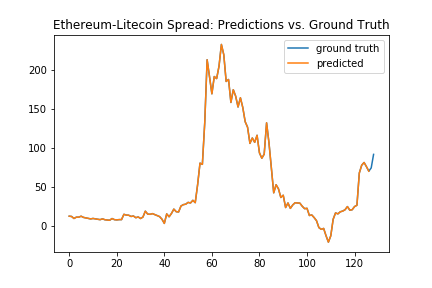
\includegraphics[scale=0.60]{/Users/jrosaler/Dropbox/Extra/"Udacity Capstone"/"Capstone Submission 3"/Test_Set_Results.png}
\caption{The final model selected by time series cross validation achieves an test set RMSE of 14.400, which does not improve upon the initial implementation score of 14.292 or the benchmark score of 14.353.} 
\label{TestResults}
\end{figure}

The file Capstone\_Main.ipynb contains plots of the 1-day forecasts of the persistence model against the ground truth values on the test set, and of the 1-day forecasts of the time series cross validated LSTM model against the ground truth values on the test set. The benchmark persistence forecast shows the characteristic lag of the predictions (orange line) against the ground truth labels (blue line). The LSTM model shows a similar lag, but its value of the RMSE on the test set indicates inferior performance as compared with the persistence forecast. 

The file Preliminary\_Tests.ipynb likewise plots the performance of a stacked LSTM model trained for 10 epochs, with batch size 200, and 64 and 32 neurons in the first and second hidden layers, respectively. The plot of the predictions (orange) overlays the plot of the ground truth values (blue), reflecting the superior performance of the LSTM model relative to the benchmark (although it should be kept in mind that the model has been tuned to the test set here).


\subsection{Reflection}

In this project, I have investigated whether LSTM neural networks may be of use in predicting the movement of price spread series of cointegrated cryptocurrency pairs. As a benchmark, a persistence forecast model was used. 

The steps of the project can be summarized as follows. Seven cryptocurrency price series were selected so as to maximize the amount of available training data while also exploring a wide range of possible pairs as candidates for cointegration. The Engle-Granger method was used to identify cointegrated pairs and compute their spread series. A single spread series, associated with the Ethereum-Litecoin spread, was then selected on the basis of its cointegration score to investigate the applicability of LSTM networks in spread prediction. The RMSE for the benchmark persistence forecast was computed on the test portion of the spread series as a benchmark value. The Ethereum-Litecoin spread data was then transformed for input into the LSTM model; these transformations included conversion to supervised format, differencing, and scaling. 

Preliminary tests experimented with single-layer and two-layer LSTM networks as well as ARIMA models. For the LSTM networks, a wide range of values for the number of training epochs, batch size, and number of neurons in each layer were tried. The best performance of the LSTM network was found to marginally surpass that of the benchmark. A grid search of the ARIMA model on the test set was also performed, again just marginally surpassing performance of the benchmark forecast. 

This preliminary testing was followed by a more rigorous analysis of the stacked LSTM model using a grid search with time series cross validation. Here, the results on the test set were found to fall just short of the benchmark model. While the results of the preliminary test managed to just barely surpass the performance of the benchmark, the results of time series cross validation are more reliable since the test set was not used to select the model hyperparameters. These results fell short of my initial expectation that the LSTM forecast would surpass the benchmark persistence forecast, although the initial implementation did this to a small degree.  

Among the most interesting aspects of this project were the strong oscillations of the cointegrated spread series about their mean, and the fact that the oscillations of different spread series all began to increase in amplitude around the same date. Also, I was surprised by fact that the LSTM model fell short of an extremely basic persistence forecast is puzzling given their success elsewhere in sequence prediction. I intend to investigate this question further in order to more clearly understand the limitations of LSTM network. The most challenging aspect of the project was training the LSTM network to give useful predictions on spread series data, a challenge that this investigation has so far not met. 

\subsection{Improvement}

The preceding analysis may be extended in various directions. 

First, they may be extended to a study of non-parametric approaches to pairs trading of co-integrated spreads. Inspection of the plots of the four co-integrated spread series suggest that it may be profitable to adopt a threshold trading strategy in which one goes long on the spread $S$ when the spread $S < \mu -  c * \sigma$ and shorts the spread when $S > \mu -  c * \sigma$, where $c$ is some constant of order one and $\sigma$ is the standard deviation of the spread series. The success of these approaches can be measured by returns, Sharpe ratio and other metrics generated on the test set. Other non-parametric approaches - for example, allowing for the possibility of different thresholds above and below the mean in the case of asymmetric mean reverting behavior - should also be investigated. 

Second, it is possible that the predictive power of the LSTM trained on past prices of the spread series would be improved by including additional indicators as input - for example, Bollinger bands, Relative Strength Index (RSI), and Moving Average Convergence Divergence (MACD). 

A third possibility is to explore the behavior of spreads formed through multivariate cointegration, as Leung \& Nguyen do. 

A fourth possibility that may be worth exploring is to restrict the training of the LSTM to only the period for which the volatility of the spread series is observed. This may help the LSTM to learn specifically those patterns in the data, which are what one hopes will generalize to future observations. 



\def\bibsection{\section*{References}}
\scriptsize
\bibliographystyle{plain}
\bibliography{References}






\end{document}